\documentclass[12pt, a4paper]{article}
\usepackage{siunitx} % For SI units
\usepackage{graphicx} % For inlcuing images.
\usepackage{float} % For H arguemnt of floats like figures.
\usepackage{booktabs} % For toprule etc. for tables
\usepackage{hyperref}
\usepackage{cleveref} % For better referencing of labels.
\begin{document}
After grinding the educts CuO, Y$_3$O$_3$ and BaCO$_3$ to a fine powder, their diffraction spectrum is measured with a X-Ray diffraction spectrometer. The resulting spectrum is seen in \Cref{fig:bs}.
\begin{figure}[H]
	\centering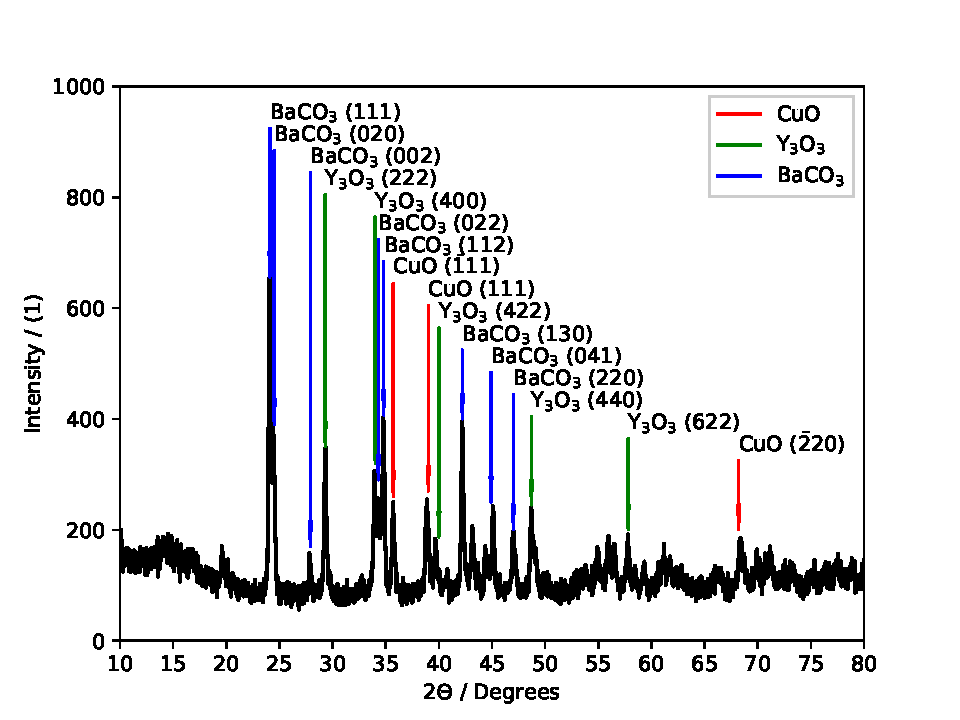
\includegraphics[width=0.8\linewidth]{../images/before_sintering_spectrum.pdf}
	\caption{Spectrum before sintering with labeld peaks for material and plane. }\label{fig:bs}
\end{figure}
A whole array of peaks can be identified. They are tabled in \Crefrange{tab:yo}{tab:baco} and can be seen on the figure. Especially for higher angles, a whole sea of tightly packed peaks are measured. As their angle only varies by up to a degree, they can not be labled with certainty, as it is very easy to confuse them with each other. Nonethereless two prominent peaks of CuO and Y$_3$O$_3$ are identified.

% ----- Y2O3 (Cubic Yttria) -----
\begin{table}[H]
	\centering
	\begin{minipage}{0.3\textwidth}
		\centering
		\begin{tabular}{cc}
			\toprule
			$2\Theta$/° & $(hkl)$ \\
			\midrule
			29.1          & $(222)$ \\
			33.8          & $(400)$ \\
			39.8          & $(422)$ \\
			48.5          & $(440)$ \\
			57.6          & $(622)$ \\
			\bottomrule
		\end{tabular}
		\caption{Standard diffraction peaks for cubic Y$_2$O$_3$}\label{tab:yo}
	\end{minipage}
	\hfill
	\begin{minipage}{0.3\textwidth}
		\centering
		\begin{tabular}{cc}
			\toprule
			$2\Theta$/° & $(hkl)$       \\
			\midrule
			35.5          & $(\bar{1}11)$ \\
			38.8          & $(111)$       \\
			68.0          & $(\bar{2}20)$ \\
			\bottomrule
		\end{tabular}
		\caption{Standard diffraction peaks for CuO}\label{tab:cuo}
	\end{minipage}
	\hfill
	\begin{minipage}{0.3\textwidth}
		\centering
		\begin{tabular}{cc}
			\toprule
			$2\Theta$/° & $(hkl)$ \\
			\midrule
			23.9          & $(111)$ \\
			24.3          & $(020)$ \\
			27.7          & $(002)$ \\
			34.6          & $(112)$ \\
			42.0          & $(130)$ \\
			44.7          & $(041)$ \\
			46.8          & $(220)$ \\
			\bottomrule
		\end{tabular}
		\caption{Standard diffraction peaks for orthorhombic BaCO$_3$}\label{tab:baco}
	\end{minipage}
\end{table}
After sintering them at \SI{950}{°C} for \SI{12}{h}, the ceramic is grinded and with diffraction measured again. As a result the spectrum of \Cref{fig:as} is obtained.
\begin{figure}[H]
	\centering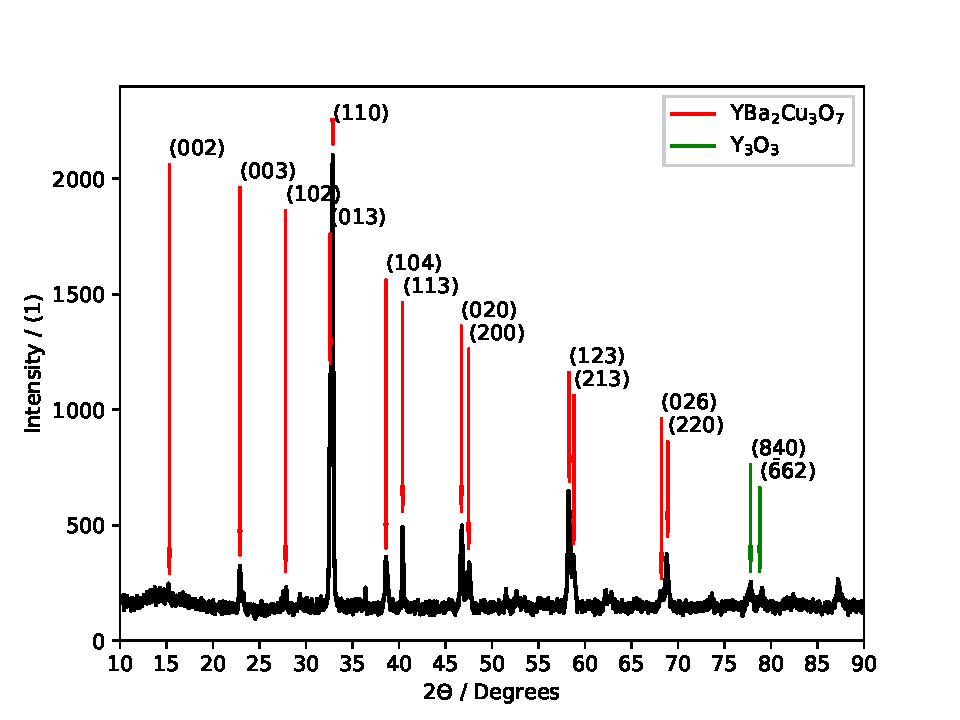
\includegraphics[width=0.8\linewidth]{../images/after_sintering_spectrum.pdf}
	\caption{Spectrum after sintering with labeld peaks for material and plane. }\label{fig:as}
\end{figure}
It can be seen that most peaks are identified with planes of the YBa$_2$Cu$_3$O$_7$ ceramic. They are tabled in \Cref{tab:ybacuo}. Some speaks for higher angles can not be assigned to the new ceramic. Instead they lie directly on two high angles diffractions peaks of the Y$_2$O$_3$ educt. This shows, that there are still some residuals that did not react yet. This can happen because larger crumbs in the mixture, i.e. the grinding process was not thorough enough, the sintering time was to short or the temperature was to low. The assigned angles are listed in \Crefrange{tab:ybacuo}{tab:highyo}. Unfortunately, the high angle peaks of Y$_2$O$_3$ can not be seen with certain in \Cref{fig:bs}, because the dense sea of diffraction peaks does not allow for differentiation, as already mentioned.



% ----- YBCO (YBa2Cu3O7, Orthorhombic) -----
\begin{table}[H]
	\centering
	\begin{minipage}{0.45\textwidth}
		\centering
		\begin{tabular}{cc}
			\toprule
			$2\Theta$/°  & $(hkl)$ \\
			\midrule
			15.3          & $(002)$ \\
			22.9          & $(003)$ \\
			27.8          & $(102)$ \\
			32.6          & $(013)$ \\
			32.9          & $(110)$ \\
			38.6          & $(104)$ \\
			40.4          & $(113)$ \\
			46.7          & $(020)$ \\
			47.5          & $(200)$ \\
			58.3          & $(123)$ \\
			58.8          & $(213)$ \\
			68.2          & $(026)$ \\
			68.9          & $(220)$ \\
			\bottomrule
		\end{tabular}
		\caption{Standard diffraction peaks for orthorhombic YBa$_2$Cu$_3$O$_7$}\label{tab:ybacuo}
	\end{minipage}
	\hfill
	\begin{minipage}{0.45\textwidth}
		\centering
		\begin{tabular}{cc}
			\toprule
			$2\Theta$/° & $(hkl)$       \\
			\midrule
			77.8          & $(840)$       \\
			78.8          & $(\bar{6}62)$ \\
			\bottomrule
		\end{tabular}
		\caption{High-angle Y$_2$O$_3$ secondary-phase peaks}\label{tab:highyo}
	\end{minipage}
\end{table}
Afterwards, using a hydraulic press, the powder is pressed into pallets and sintered again. The final product is the high-temperature superconductor YBa$_2$Cu$_3$O$_7$.



\end{document}
